
% =========================================================================
% SECTION: CONTROL SYSTEM DESIGN FOR DC-DC CONVERTERS
% =========================================================================
\section{Control System Design for DC-DC Converters}

In an Electric Vehicle charging station integrated with Photovoltaic arrays, DC-DC converters must constantly adjust to shifting power demands. Because internal parts possess inherent electrical resistance, an increase in current causes the output voltage to naturally sag, potentially destabilizing the system. To solve this, a closed-loop feedback mechanism monitors these fluctuations and automatically widens the pulse-width modulation signals. This corrective action ensures the device maintains a consistent target voltage or current despite the dynamic and unpredictable nature of the connected load.

\subsection{Analytical Design vs. Trial-and-Error}
Utilizing mathematical modelling paired with deterministic frequency-response design offers an absolute engineering advantage over empirical ``trial-and-error'' tuning methods:

\begin{itemize}
    \item \textbf{Parametric Flexibility \& Scalability:} The control loop is completely parameterized. If any physical component changes (e.g., $R$, $L$, or $C$), you simply update the parameter value.
    \item \textbf{Rapid Re-Execution (Automated Scripting):} The entire script executes instantly to recalculate precise analog gains ($K_p$, $\omega_c$) and digital coefficients ($b_0$, $b_1$, $a_1$). This minimizes development cycle times.
\end{itemize}

\subsection{Voltage/Current Loop Control Design}
The closed-loop voltage control loop is designed systematically using the frequency response (loop-shaping) method. The entire procedure transitions from continuous-time analytical tuning to discrete difference equations ready for microcontroller firmware.

\newpage

\subsubsection{Hardware \& System Parameter Configurations}
The system configuration and open-loop transfer function variable initialization calculations are executed via the script setup below:

\begin{lstlisting}
%% circuit parameters
R = 10;          % Load resistance in ohms
rL = 1.9;        % Inductor resistance in ohms
rC = 0.2;        % Capacitor equivalent series resistance in ohms
Vo = 3.8;        % Output voltage in volts
Vin = 12.3;      % Input voltage in volts
rDS = 0.025;     % On-resistance of the switch in ohms
Vfwd = 0.8;      % Forward voltage drop of the diode in volts

%% Calculate the load current
Io = Vo / R;     % Output current in amps

%% Calculate the inductor current
iL = Io;         % Inductor current in amps

%% Calculate the duty cycle
Du = (Vfwd + iL * rL + Vo) / (Vin - iL * rDS + Vfwd);

%% Define the ripple specs
delta_iL = 0.6 * iL;     % Inductor current ripple in amps
delta_Vo = 0.02 * Vo;    % Output voltage ripple in volts

%% the switching frequency
fsw = 10e3;

%% the stress on components
Vd_stress = -Vin + iL * rDS;  % Diode stress voltage
Vsw_stress = Vin + Vfwd;      % Switch stress voltage
Id_stress = Io;               % Diode stress current
Isw_stress = Io;              % Switch stress current

%% inductance and capacitance values in design
L = 2e-3;
C = 220e-6;

%% Define the transfer function variable and plant GVdO
s = tf('s');
GVdO = (R * (C * rC * s + 1) * (Vfwd + Vin - iL * rDS)) / ...
       ((R + rL + Du * rDS + L * s + C * L * R * s^2 + ...
       C * L * rC * s^2 + C * R * rC * s + C * R * rL * s + ...
       C * rC * rL * s + C * Du * R * rDS * s + C * Du * rC * rDS * s));
\end{lstlisting}

\subsubsection{Frequency Response Specs: Phase Margin \& Crossover Frequency}

We begin by designing via the frequency response of the system, setting two main constraints: our desired phase margin and the target crossover frequency.

\begin{lstlisting}
%% Frequency Response Specs: Phase Margin & Crossover Frequency
CROSS_FREQ = 200;   % Crossover frequency in rad/s
des_PM = 90;        % Desired phase margin
fc_v = (CROSS_FREQ) / (2 * pi); % Crossover frequency
wc_v = CROSS_FREQ;

% Calculate the target phase margin in radians
targ_PM_v = deg2rad(des_PM);
\end{lstlisting}

\subsubsection{Evaluate Plant Phase at Crossover Frequency}
We want to compute the phase of the plant. We utilize the system's analytical plant transfer function ($G_{V_oD}$) to do this.

\begin{lstlisting}
%% Evaluate Plant Phase at Crossover Frequency
% Define the transfer function variable and plant GVdO
s = tf('s');
GVdO = (R * (C * rC * s + 1) * (Vfwd + Vin - iL * rDS)) / ...
       ((R + rL + Du * rDS + L * s + C * L * R * s^2 + ...
       C * L * rC * s^2 + C * R * rC * s + C * R * rL * s + ...
       C * rC * rL * s + C * Du * R * rDS * s + C * Du * rC * rDS * s));

% Evaluate the transfer function at the crossover frequency
gpc_v = evalfr(GVdO, wc_v * 1i);

% Calculate the gain and phase at the crossover frequency
gain_v = abs(gpc_v);
phase_v = angle(gpc_v);
\end{lstlisting}

\subsubsection{Determine Phase Compensation}
By subtracting the plant's phase from your target margin, you determine the required phase compensation ($pc\_v$). Since the resulting value is highly negative ($\approx -83.96^\circ$), it dictates a lag compensator profile.

\begin{lstlisting}
%% Determine Phase Compensation
% Calculate the phase compensation
pc_v = targ_PM_v - phase_v - pi;
\end{lstlisting}

\subsubsection{Calculate Integral and Proportional Components}
We calculate the integral component, then via trigonometric substitution, we calculate the proportional component while taking the overall plant gain into account. This solves for our two unknowns in our analog PI controller equation:

\begin{equation}
    G_c(s) = K_p \left( \frac{\omega_i}{s} + 1 \right)
\end{equation}

\begin{lstlisting}
%% Calculate Integral and Proportional Components
% Calculate the integral component
fi_v = -fc_v * tan(1 * pc_v);

% Calculate the proportional gain
Kp_v = (1 / gain_v) / sqrt((fi_v / fc_v)^2 + 1);

% Integral component in rad/s
wi_v = fi_v * 2 * pi;

% Define the compensator transfer function Gc_v
Gc_v = Kp_v * ((wi_v / s) + 1);
\end{lstlisting}

\subsubsection{Discretization via Bilinear Z-Transform}
Since this is an analog transfer function in the continuous $s$-domain, we need to transform it to the digital $z$-domain to run on a finite-time microcontroller. We apply the Bilinear Z-Transform:

\begin{equation}
    s = \frac{2}{T_s} \frac{z - 1}{z + 1}
\end{equation}

with a sampling frequency of 10 kHz ($T_s = \frac{1}{10000} = 100\ \mu\text{s}$). This maps our continuous poles and zeros into the discrete domain, yielding the digital transfer function coefficients ($b_0$, $b_1$, $a_1$).

\begin{lstlisting}
%% Discretization via Bilinear Z-Transform
% Discretize the compensator and open-loop transfer functions
Gc_v_d = c2d(Gc_v, 100);
\end{lstlisting}

\subsubsection{Stability Verification}
We view the closed-loop step response of our newly discretized system to make absolutely sure it remains stable, tracking the transient characteristics correctly before physical hardware deployment.

\begin{lstlisting}
%% Stability Verification
% step response of the closed-loop system
step(feedback(T_v_d, 1), 0.1);
\end{lstlisting}

\begin{figure}[H]
    \centering
    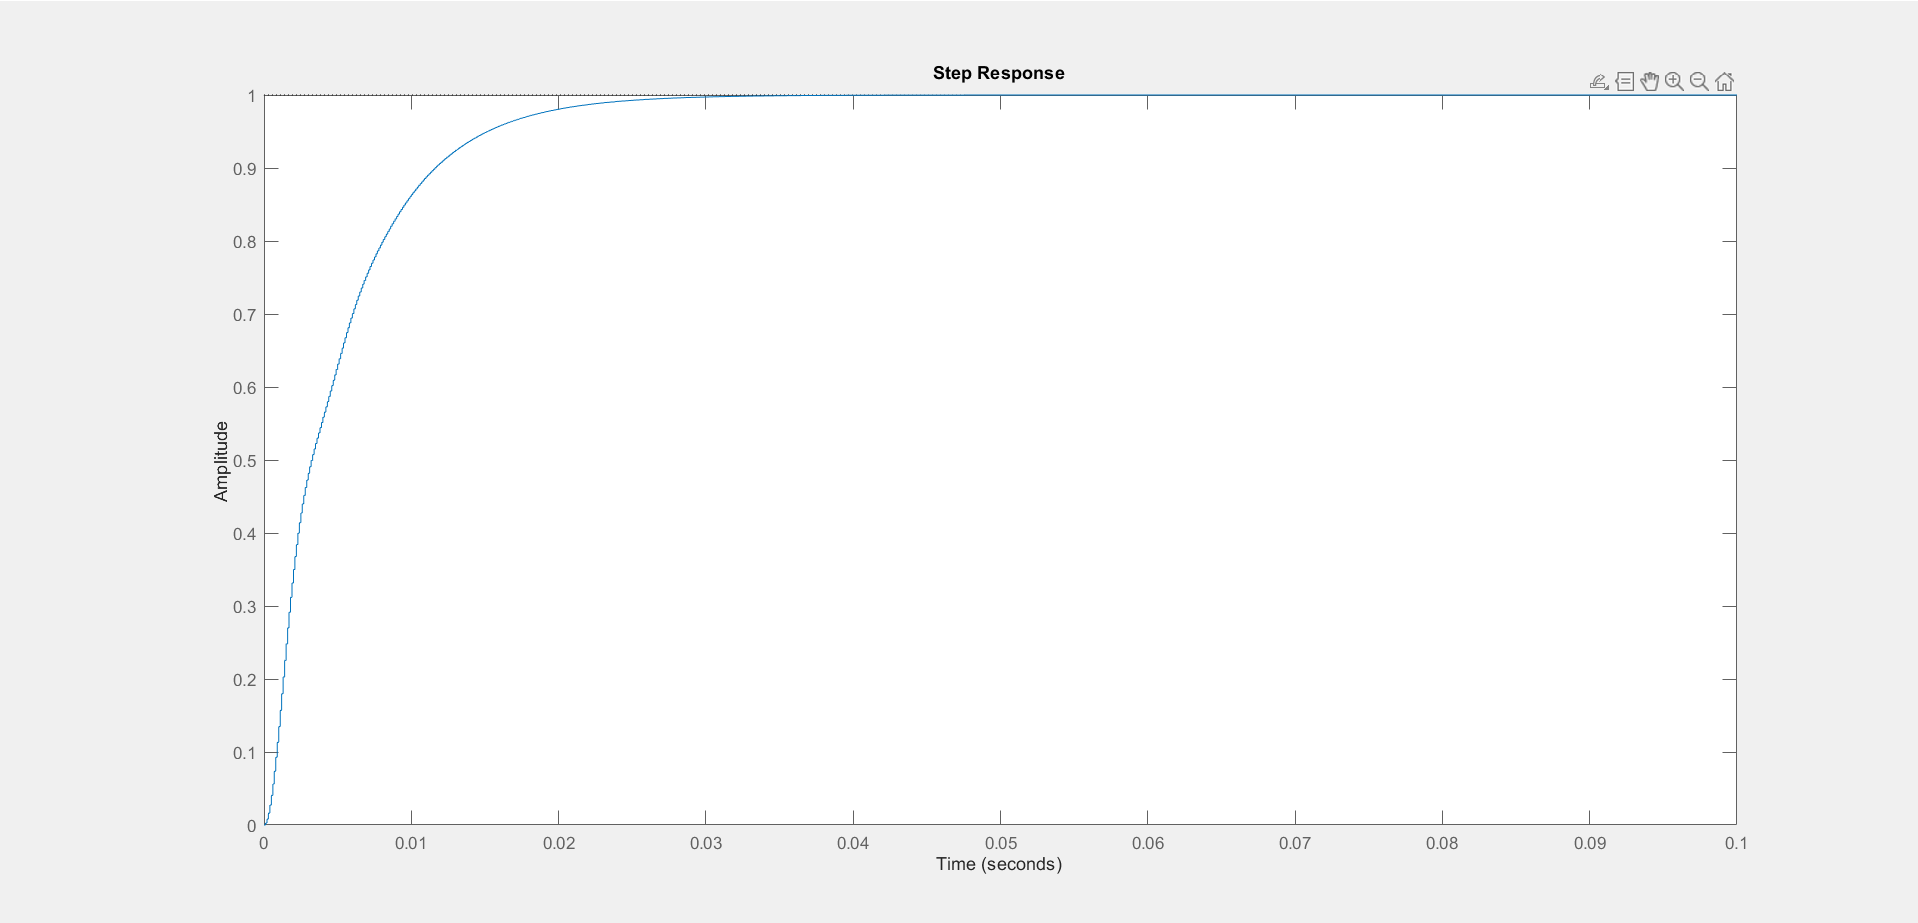
\includegraphics[width=0.9\textwidth]{Figures/step_response.png}
    \caption{Closed-loop system digital step response tracking.}
    \label{fig:control_step_response}
\end{figure}

\subsubsection{Frequency Response \& Stability Analysis (Bode Plot)}
We plot the Bode response of our system to verify the tracking performance, gain margin, and phase margin criteria under both continuous and discretized loop conditions.

\begin{lstlisting}
%% Frequency Response & Stability Analysis (Bode Plot)
% Bode plots for the transfer functions
margin(GVdO);    % Uncompensated Plant
margin(T_v);     % Continuous-time Open-Loop System
margin(T_v_d);   % Discretized Open-Loop System
\end{lstlisting}

\begin{figure}[H]
    \centering
    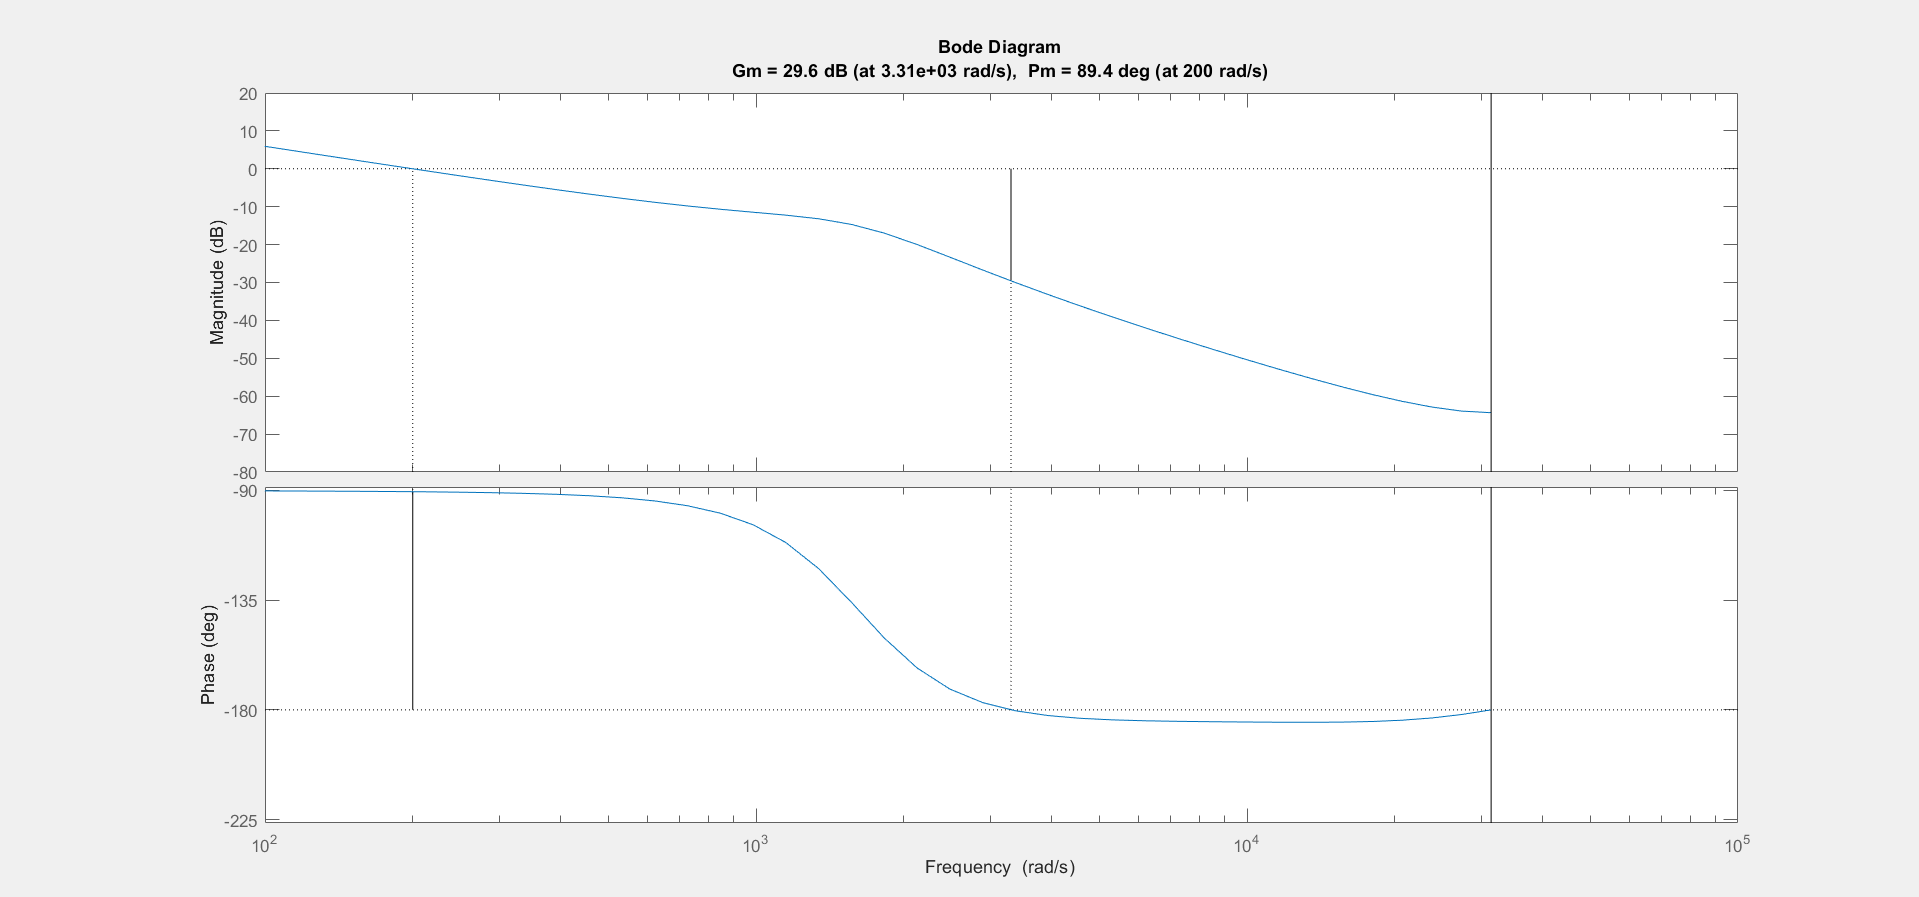
\includegraphics[width=0.9\textwidth]{Figures/bode_plot.png}
    \caption{System Bode diagram highlighting phase and gain margins.}
    \label{fig:control_bode_plot}
\end{figure}